\documentclass[aspectratio=169]{beamer}
%
% Choose how your presentation looks.
%
% For more themes, color themes and font themes, see:
% http://deic.uab.es/~iblanes/beamer_gallery/index_by_theme.html
%
\mode<presentation>
{
  \usetheme{Berlin}      % or try Darmstadt, Madrid, Warsaw, ...
  \colorlet{beamer@blendedblue}{green!80!black!80!blue!80}
  \setbeamercolor{normal text}{fg=white,bg=darkgray}
  \usefonttheme{default}  % or try serif, structurebold, ...
  \setbeamertemplate{navigation symbols}{}
  \setbeamertemplate{caption}{\raggedright\insertcaption\par}
} 

\usepackage[czech]{babel}
\usepackage[utf8]{inputenc}
\usepackage{graphicx}
\usepackage{movie15}
\usepackage{caption}
\usepackage{subcaption}
\usepackage{listings}
\graphicspath{ {./imgs/} }

\title[Klasifikace lomů]{\textbf{Klasifikace lomů}}
\author{Plajta}
\institute{VOŠ a SPŠE Plzeň}
\date{\today}

\begin{document}

\captionsetup[subfigure]{labelformat=empty}
\captionsetup{labelformat=empty}

\begin{frame}
  \titlepage
\end{frame}

% Uncomment these lines for an automatically generated outline.
%\begin{frame}{Outline}
%  \tableofcontents
%\end{frame}

\section{Úvod}

\subsection{Lomy}

\begin{frame}{Lomy}
    \begin{figure}
        \centering
        \includegraphics[height=5.5cm]{lom.png}
    \end{figure}
\end{frame}

\begin{frame}{Opravdu Lomy}
    \begin{figure}
        \centering
        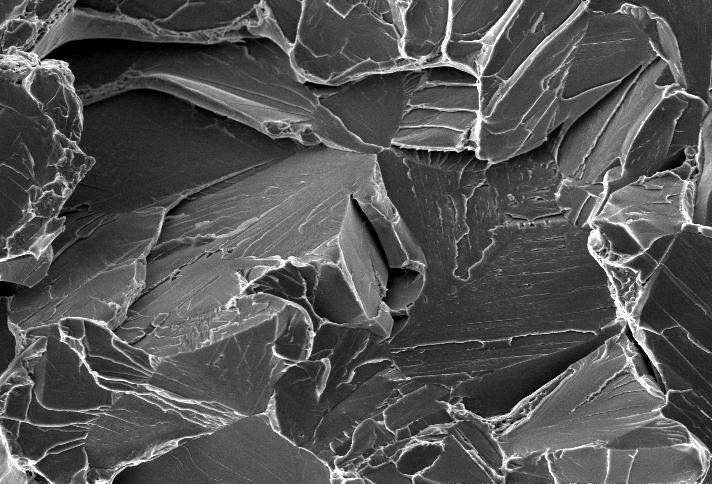
\includegraphics[height=5.5cm]{stepny.png}
    \end{figure}
\end{frame}

\section{Data loader}

\begin{frame}{Data loader}
    \begin{figure}
        \centering
        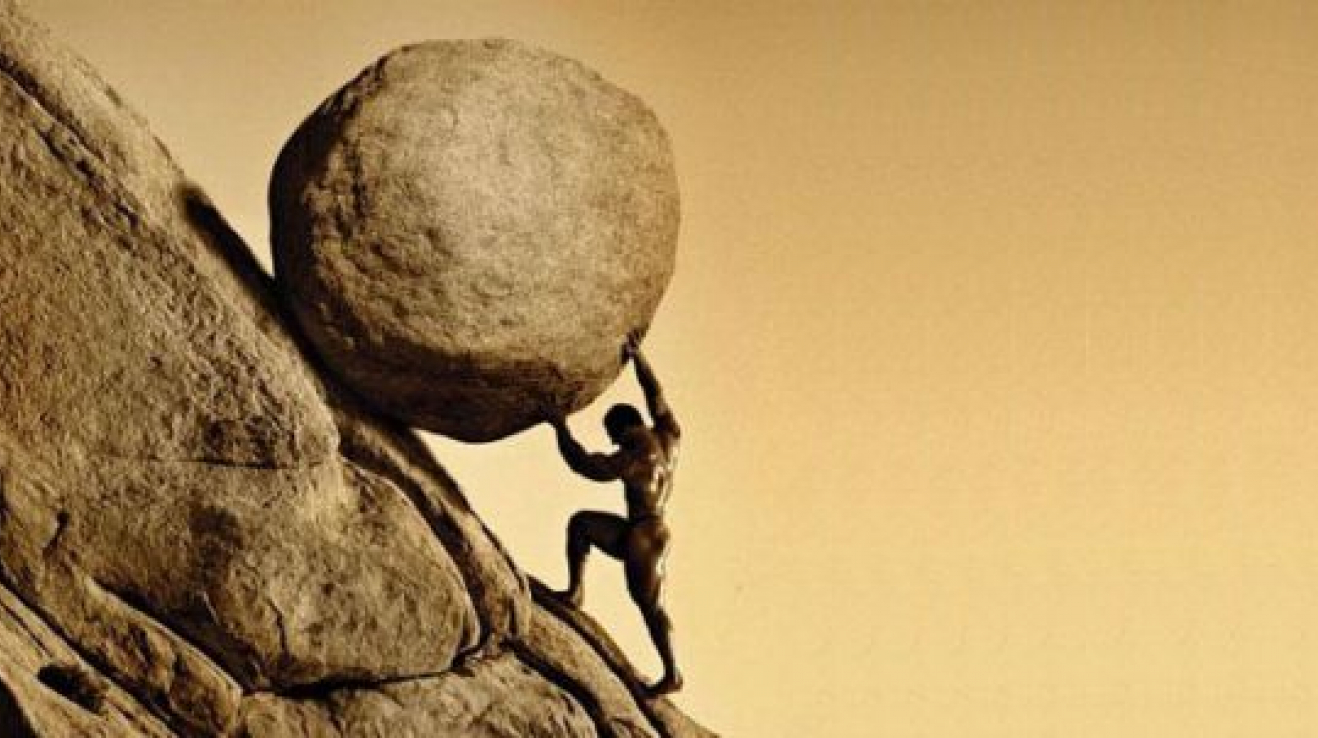
\includegraphics[height=5.5cm]{sisyfos.jpg}
    \end{figure}
\end{frame}

\section{Klasické modely strojového učení}

\subsection{SVC}

\begin{frame}{SVC}
    \begin{itemize}
        \item C-Support Vector Classification
    \end{itemize}
    \begin{figure}
        \centering
        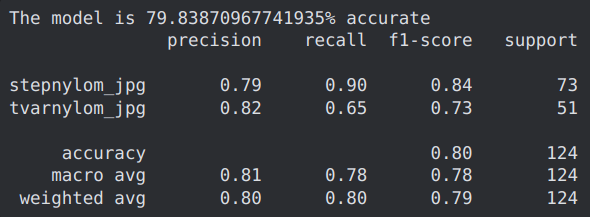
\includegraphics[height=4cm]{SVC_table.png}
        \caption{Evaluační metriky SVC}
    \end{figure}
\end{frame}

\subsection{KNN}

\begin{frame}{KNN}
    \begin{itemize}
        \item K-Nearest Neighbors
    \end{itemize}
    \begin{figure}
        \centering
        \begin{subfigure}{.5\textwidth}
            \centering
            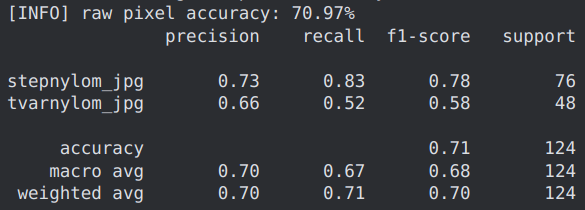
\includegraphics[height=2.4cm]{KNNr_table.png}
            \caption{Evaluační metriky KNN ze surových dat}
            \label{fig:sub1}
        \end{subfigure}%
        \begin{subfigure}{.5\textwidth}
            \centering
            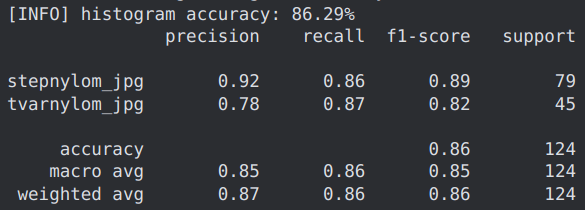
\includegraphics[height=2.4cm]{KNNh_table.png}
            \caption{Evaluační metriky KNN z histogramu}
            \label{fig:sub2}
        \end{subfigure}
    \end{figure}
\end{frame}

\section{Neuronové sítě}

\subsection{Pytorch}

\begin{frame}{Pytorch}
    \begin{itemize}
        \item Snaha byla...
    \end{itemize}
    \begin{figure}
        \centering
        \includegraphics[height=4cm]{we_really_tried.png}
        \caption{*představte si snahu*}
    \end{figure}
\end{frame}
\subsection{Tensorflow - Keras}

\begin{frame}{Tensorflow - Keras}
    Neuronové sítě:
    \begin{itemize}
        \item CNN
        \item Ensemble CNN
    \end{itemize}
    \begin{figure}
        \centering
        \begin{subfigure}{.5\textwidth}
            \centering
            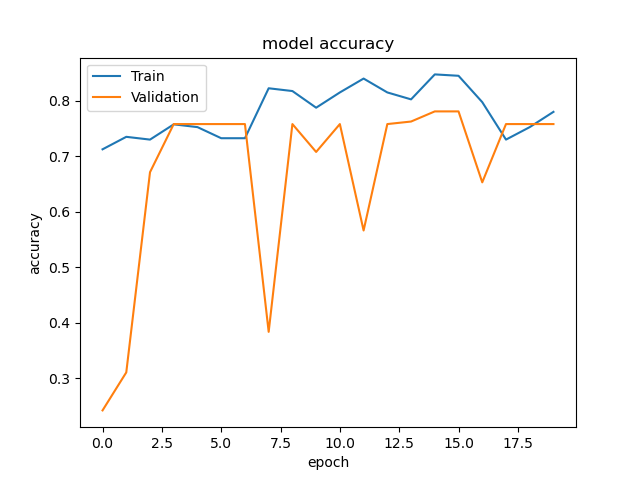
\includegraphics[height=3.8cm]{accuracy_b_size8.png}
            \caption{Přesnost modelu}
            \label{fig:sub1}
        \end{subfigure}%
        \begin{subfigure}{.5\textwidth}
            \centering
            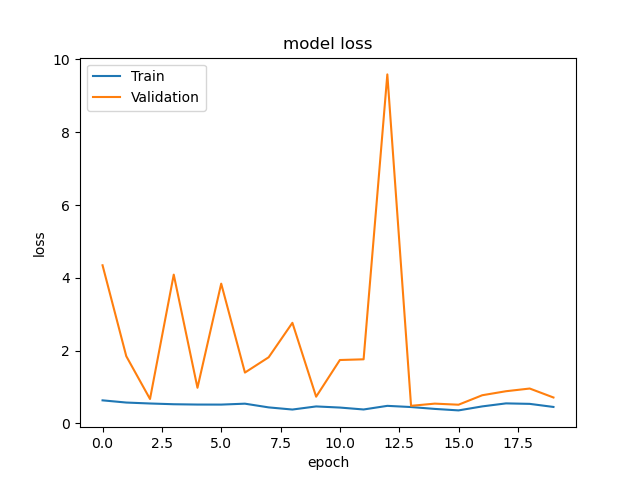
\includegraphics[height=3.8cm]{loss_b_size8.png}
            \caption{Ztráta modelu}
            \label{fig:sub2}
        \end{subfigure}
    \end{figure}
\end{frame}

\begin{frame}{Tensorflow - Keras}
    \begin{figure}
        \centering
        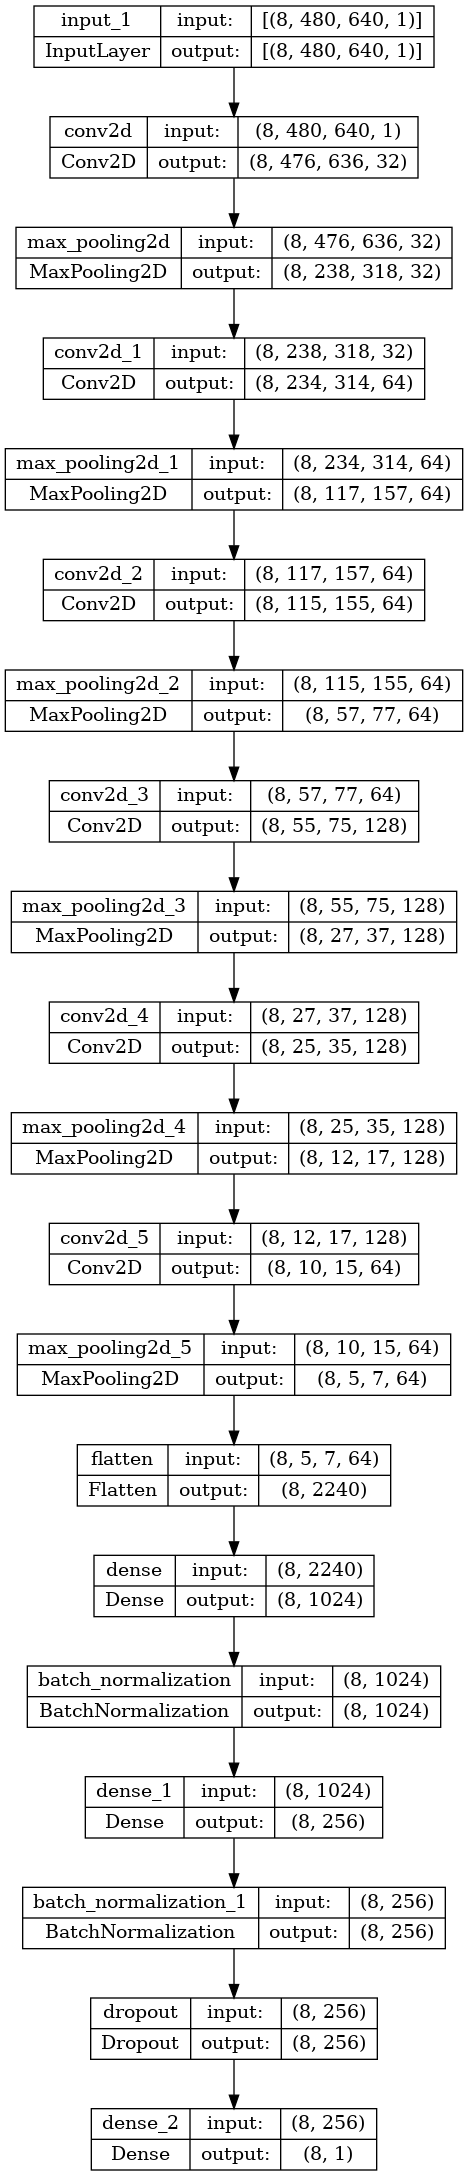
\includegraphics[trim={0 51cm 0 0},clip,width=3.8cm]{model_plot.png} \hfill
        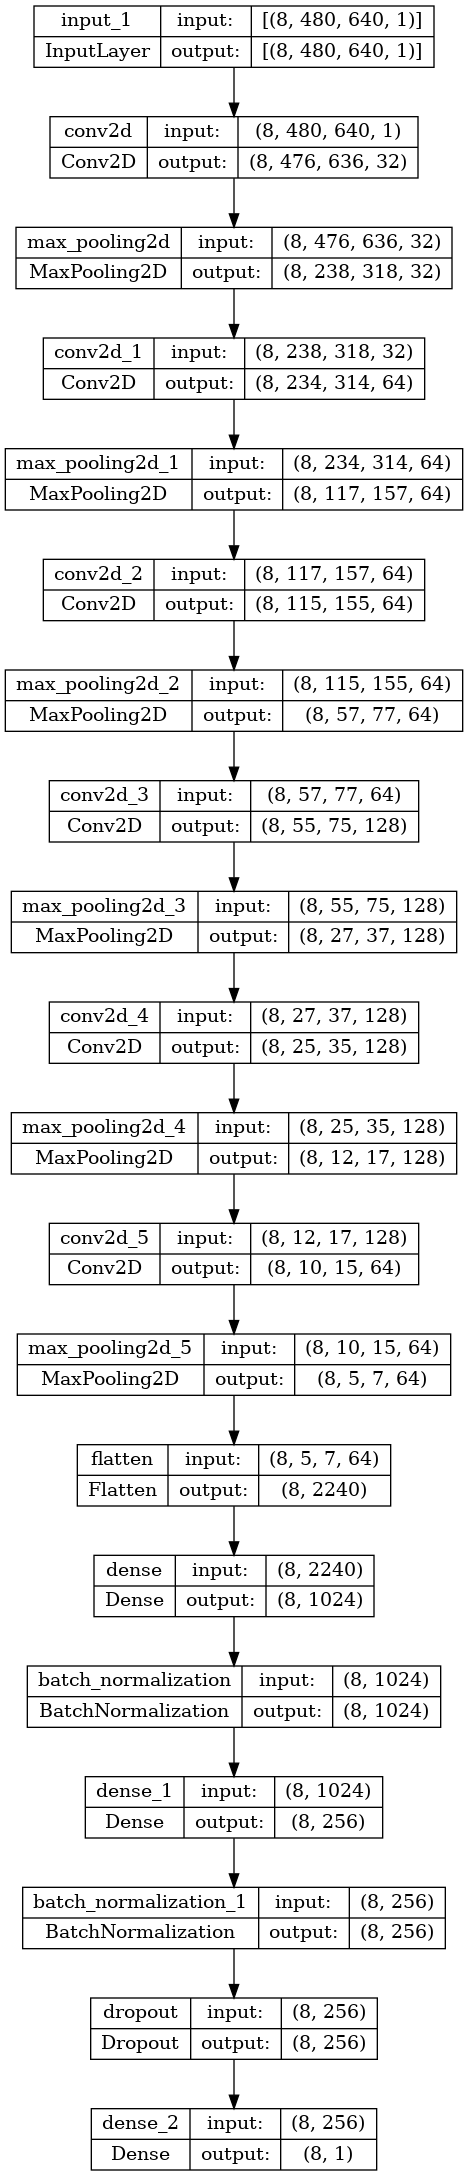
\includegraphics[trim={0 25.5cm 0 25.5cm},clip,width=3.8cm]{model_plot.png} \hfill
        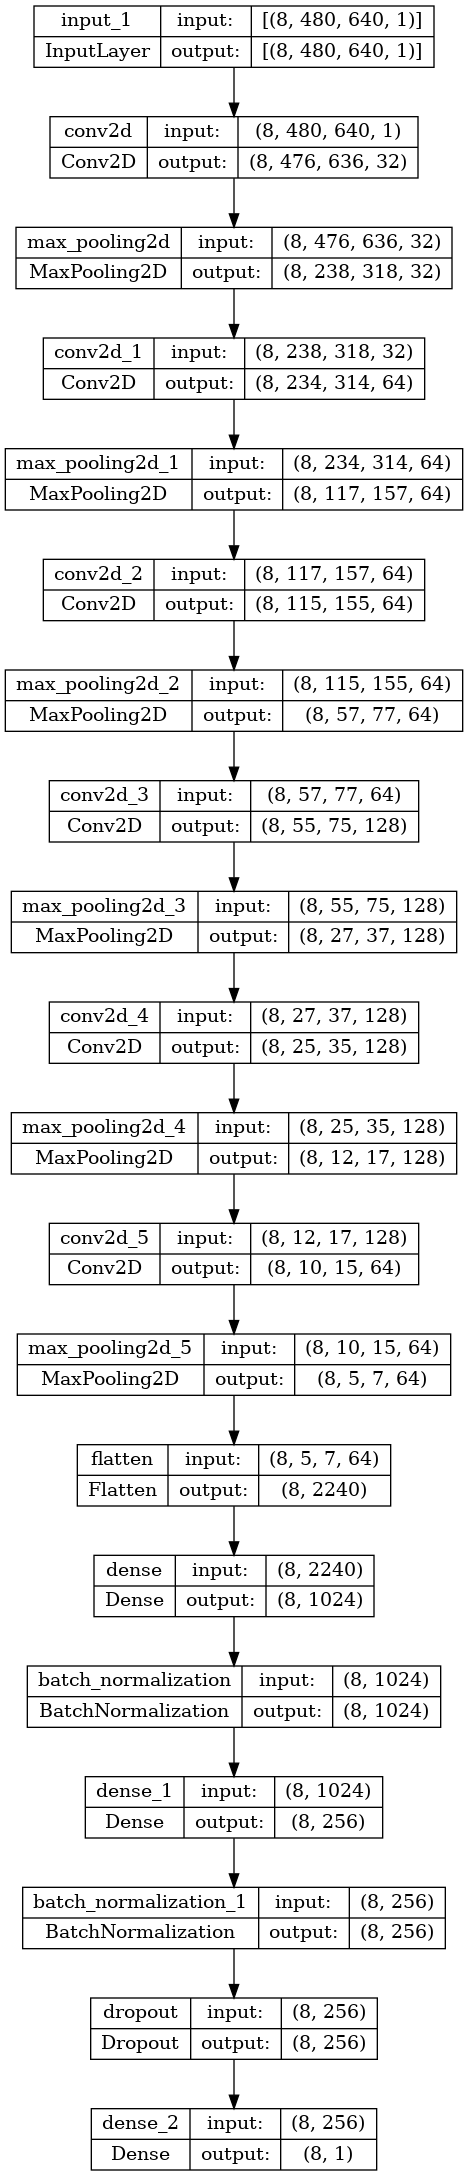
\includegraphics[trim={0 0 0 51cm},clip,width=3.8cm]{model_plot.png} \hfill
    \end{figure}
\end{frame}

\section{GUI}

\subsection{Tkinter}

\begin{frame}{Tkinter}
    \begin{itemize}
        \item Jednoduché a relativně multiplatformní
    \end{itemize}
    \begin{figure}
        \centering
        \includegraphics[height=4cm]{images/send_solution.png}
        \caption{GUI pro naše modely}
    \end{figure}
\end{frame}

\subsection{Závěr}

\begin{frame}{Závěr}
    \begin{itemize}
        \item Vyzkoušeli jsme více způsobů
        \item Přemýšleli jsme o voting systému
    \end{itemize}
    \begin{figure}
        \centering
        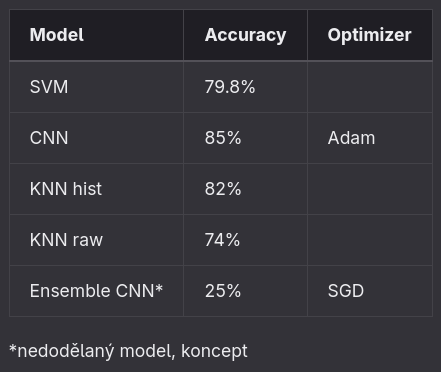
\includegraphics[height=4cm]{table.png}
        \caption{Shrnutí přesností algoritmů}
    \end{figure}
\end{frame}

\end{document}
